
%: ----------------------- physics file header -----------------------
\chapter{Overview of Relevant Physics}

% the code below specifies where the figures are stored
\ifpdf
    \graphicspath{{physics/figures/PNG/}{physics/figures/PDF/}{physics/figures/}}
\else
    \graphicspath{{physics/figures/EPS/}{physics/figures/}}
\fi

% ----------------------------------------------------------------------
% ----------------------- Physics content -------------------------
% ----------------------------------------------------------------------
\section{The Standard Model}
The standard model of particle physics is our current best way of understanding
all particle interactions that have so far been observed.
It's defining aspect is as a gauge theory in which all interactions
preserve a local $SU{(3)}_C \times SU{(2)}_L \times U{(1)}_Y$ symmetry, where
$C$, $L$, and $Y$ respectively indicate color, left-hand chirality and weak hyperchange.
These symmetry groups specify the number of bosons that mediate each...

The $SU({(3)}_C$ symmetry corresponds to the strong nuclear force and quark/gluon
interactions.

\section{Neutrinos}
Neutrinos were first hypothesized by Wolfgang Pauli in 1930.
The motivation for the proposal the apparent violation of energy
conservation in $\beta$ decay \citep{pauli_letter}.
Several years after Pauli's speculative proposal Enrico Fermi offered
a thorough model of beta decay that conserved energy using the neutrino
\citep{fermi_beta_decay}.
%Fermi's model predicted such a small cross-section for the neutrino that some
%doubted it would ever be observed \citep{bethe_impossible_to_observe}.
Nearly two decades after its initial proposal, Frederick Reines \&
Clyde Cowan performed an experiment that involved bombarding a tank of cadmium
doped water with anti-neutrinos from nuclear reactor~\cite{cowan_reines}.
Their detector was able to observe the rate and energy of inverse $\beta$
decays that occurred.
The experiment's results were consistent with Fermi's model of $\beta$ decay and were
considered a confirmation of the neutrino's existence.

The first experimental evidence for neutrino flavor came in 1962 from an
experiment \citep{lederman_muon_flavor} that studied the interactions of
neutrinos that came from muon decay, and the interactions of neutrinos
from beta decay.
The experiment observed that neutrinos from came from muon decay would produce
muons upon interacting in a detector.
And neutrinos produced from $\beta$ decay would create electrons in the
detector.
This lead to the conclusion that there are two different varieties of neutrino,
the $\nu_e$ and the $\nu_{\mu}$, and the idea that lepton flavor is conserved in
Weak interactions.
The third lepton generation, the $\tau$ and the $\nu_{\tau}$ was discovered 13
years later in 1975 \citep{tau_discovery}.
% It's worth noting that lepton flavor conservation was not predicted or required
% by the standard model, for that reason it's known as an 'accidental symmetry'.
% ^^^^Not true??? Lepton number is an accidental symmetry, idk about lepton
% flavor Also the definition of accidental symmetry has to do with term in the
% lagrangian being to high dimensional (according to wikipedia) not what I
% said....though they might be the same somehow

\subsection{Neutrino Interactions}
The neutrino interacts almost exclusively via the weak interaction.
In principle neutrinos also interacts gravitationally and they have a non-vanishing
magnetic moment so can interact electromagnetically, but these
interaction potentials are so small they can be neglected in all practical
cases~\cite{neutrino_magmom}.
The weak interaction has a number of aspects that limit the sort of neutrino
interactions that can occur. One aspect is lepton flavor conservation,
all weak interactions conserve both the total lepton number of a system, but also
the total lepton flavor of the system as well.
This leads to nearly all interactions involving a neutrino also involving the
same flavor charged lepton.
The second aspect is that the weak interaction is known to be chiral,
only left-handed particles and right-handed anti-particles interact weakly.
Since neutrinos only interact weakly, the only detectable varieties of neutrino
is the left-handed neutrino $\nu^{L}$  and the right-handed
anti-neutrino $\overline{\nu}^{R}$~/cite{weinberg}.

Discussed here are the neutrino interactions occur in the energy regime
relevant for solar neutrinos.
At higher energies, $E_{\nu} \gtrapprox 100$\,MeV, neutrinos can interact
with nuclear targets through quasi-elastic scattering, resonant
pion-production, or deep inelastic scattering.
A more complete overview of neutrino interactions is available in Ref.~\cite{neutrino_xsec}.

\begin{figure}[htbp]
\centering
\begin{feynman}
\fermion[label=$\overline{\nu}_{e}$]{0.00, 0.00}{1.50, 1.00}
\fermion[label=$p$]{3.00, 0.00}{1.50, 1.00}
\electroweak[label=$W^{+}$]{1.50, 1.00}{1.5, 2.00}
\fermion[label=$e^{+}$]{1.50, 2.00}{0.0, 3.00}
\fermion[label=$n$]{1.5, 2.00}{3.00, 3.00}
\end{feynman}
\caption[Inverse Beta Decay Feynman Diagram]{Feynman diagram for the 
inverse beta decay process.}
\label{fig:ibd}
\end{figure}
At lower energies one of the most common methods for detecting (anti)neutrinos
is through inverse beta-decay (IBD), $\overline{\nu}_{e} + p \rightarrow n + e^{+}$.
Figure~\ref{fig:ibd} shows the Feynman diagram for this process.
The Cowan \& Reines experiment used this interaction to establish the existence
of the neutrino and reactor neutrino experiments still use this interaction as
their primary detection method~\cite{double_chooz1, daya_bay, reno}.
These experiments take advantage of the fact that the IBD positron and neutron
will both interact in their detector, producing a pair
of events with a known, typically very short, time delay.
By looking for pairs of events instead of a single interaction almost
all backgrounds can be removed.

\begin{figure}[htbp]
\centering
\begin{subfigure}[b]{0.48\textwidth}
\begin{feynman}
\fermion[label=$e^{-}$]{0.00, 0.00}{1.00, 1.00}
\fermion[label=$\nu_{e}$]{1.00, 1.00}{0.00, 2.00}
\electroweak[label=$W^{+}$]{1.00, 1.00}{2.0, 1.00}
\fermion[label=$n$]{3.00, 0.00}{2.0, 1.00}
\fermion[label=$p$, showArrow=true]{2.0, 1.00}{3.00, 2.00}
\end{feynman}
\caption[]{}
\label{fig:nuclear_cc}
\end{subfigure}
\hfill
\begin{subfigure}[b]{0.48\textwidth}
\begin{feynman}
\fermion[label=$e^{-}$]{0.00, 0.00}{1.00, 1.00}
\fermion[label=$\nu_{e}$]{1.00, 1.00}{0.00, 2.00}
\electroweak[label=$Z$]{1.00, 1.00}{2.0, 1.00}
    \fermion[label=$p\mathrm{,}n$]{3.00, 0.00}{2.0, 1.00}
    \fermion[label=$p\mathrm{,}n$, showArrow=true]{2.0, 1.00}{3.00, 2.00}
\end{feynman}
\caption[]{}
\label{fig:nuclear_nc}
\end{subfigure}
\caption[Neutrino Nuclear Interactions]{}
\label{fig:nuclear_interactions}
\end{figure}

Also significant at lower energies is the charged current (CC) nuclear interaction
$\nu_{e}$~$+$~$n$~$\rightarrow$~$p$~$+$~$e^{-}$.
Figure~\ref{fig:nuclear_cc} gives the Feynman diagram for this process.
The charged current nuclear interaction played a significant role in early
radio-chemical solar neutrino experiments~\cite{homestake, sage, gallex, gno}.
The Sudbury Neutrino Observatory (SNO) made use of the charged current
nuclear interaction and the similar neutral current (NC) interaction (Fig~\ref{fig:nuclear_nc})
to solve the Solar Neutrino Problem\cite{solar_nu_problem, sno_second}.
SNO and its measurements will be discussed in greater detail in Sec~\ref{sec:sno}.

\label{sec:esxsec}
% ES diagrams
\begin{figure}
\centering
\begin{subfigure}[t]{0.48\textwidth}
\centering
\begin{feynman}
\fermion[label=$e^{-}$]{0.00, 0.00}{0.80, 0.80}
\fermion[label=$\nu_{e}$]{0.80, 0.80}{0.00, 1.60}
\electroweak[label=$W^{+}$]{0.80, 0.80}{2.0, 0.80}
\fermion[label=$\nu_{e}$]{2.80, 0.00}{2.0, 0.80}
\fermion[label=$e^{-}$, showArrow=true]{2.0, 0.80}{2.80, 1.60}
\end{feynman}
\caption[Charged Current Elastic Scattering Feynman Diagram]{
Charged current elastic scattering interaction}
\label{fig:ES_CC}
\end{subfigure}
\hfill
\begin{subfigure}[t]{0.48\textwidth}
\centering
\begin{feynman}
\fermion[label=$\nu_{x}$]{0.00, 0.00}{0.80, 0.80}
\fermion[label=$\nu_{x}$]{0.80, 0.80}{0.00, 1.60}
\electroweak[label=$Z$]{0.80, 0.80}{2.0, 0.80}
\fermion[label=$e^{-}$, flip=true]{2.00, 0.80}{2.8, 0.00}
\fermion[label=$e^{-}$, showArrow=true ]{2.0, 0.80}{2.80, 1.60}
\end{feynman}
\caption[Neutral Current Elastic Scattering Feynman Diagram]{
Neutral current elastic scattering interaction}
\label{fig:ES_NC}
\end{subfigure}
\label{fig:feynman_es}
\caption[Elastic Scattering Feynman Diagrams]{The Feynman diagrams for the
    charged current elastic scattering interaction\,(a) and the neutral
    current elastic scattering interaction\,(b).}
\end{figure}

Neutrino-electron elastic scattering (ES) is an important neutrino interaction
channel for this work --- it is the main interaction through which neutrinos are
detected in Chapter~\ref{sec:sigex}.
The ES process is $\nu_{\mathrm{x}} + e^{-} \rightarrow \nu_{\mathrm{x}} +e^{-}$
or $\overline{\nu}_{\mathrm{x}} + e^{-} \rightarrow \overline{\nu}_{\mathrm{x}} +e^{-}$.
The tree level Feynman diagrams for the charged current neutrino elastic scattering
interaction is shown in Fig.~\ref{fig:ES_CC} and the neutral current elastic
scattering interaction in Fig.~\ref{fig:ES_NC}.
The neutral current interaction involves $\nu_{\mathrm{x}}$ where $x=\mathrm{e, \mu, \tau}$,
and the charged current interaction involves only $\nu_{\mathrm{e}}$.

The charged current interaction is in principle available to neutrinos of all
flavors, however, for solar neutrinos only the electron flavor version of the
interaction is available.
The initial electron on the left hand side of the interaction is usually understood to
be from an atom within target the detector, and therefore at rest within
the lab frame.
So the total energy in the interaction is simply $E = E_{\nu} + m_{e}$.
For even the highest energy solar neutrinos $E<20$\,MeV, far less that muon
rest mass of $m_{\mu}=105.7$\,MeV/$\text{c}^{2}$ or tau mass $m_\tau = 1776.8$\,MeV/$\text{c}^{2}$.
Meaning a muon or tau cannot be created; the electron with a rest mass
of $m_{e}=0.511$\,MeV/$\text{c}^{2}$ is the only charged lepton that can
be created from the CC-ES interaction for solar neutrinos.
And since lepton flavor is conserved in weak interactions, the electron neutrino
is the only neutrino that can produce an electron, therefore the electron
neutrino is the only neutrino flavor that can undergo the charged-current
elastic scattering interaction.


This flavor disparity in the interaction means that the cross-section for the
elastic scattering process is larger for $\nu_{e}$ than it is for a $\nu_\mu$
or $\nu_\tau$, and the cross-section for a $\nu_\mu$ is the same as that for a
$\nu_\tau$.
The differential cross section of for the diagrams shown in Fig~\ref{fig:ES_CC} and
Fig.~\ref{fig:ES_NC} can be calculated as
\begin{equation}
    \frac{d\sigma}{dT_{\mathrm{e}}}\left(E_{\nu}\text{, }T_{\mathrm{e}}\right)=
    \frac{\sigma_{0}}{m_{\mathrm{e}}}\left[g_{1}^{2} + g_{2}^{2}\left(1 - \frac{T_{\mathrm{e}}}{E_{\nu}}\right)^{2} -g_{1}g_{2}\frac{m_{\mathrm{e}}T_{\mathrm{e}}}{E_{\nu}^{2}}\right]\text{,}
\end{equation}
where,
\begin{equation}
    \sigma_{0} = \frac{2G^{2}_{\mathrm{F}}m_{\mathrm{e}}^{2}}{\pi}\text{.}
\end{equation}
For $\nu_{x} = \nu_{e}$
\begin{equation}
    g_{1} = \frac{1}{2} + \sin^{2}\theta_{\mathrm{W}}\text{,}
\end{equation}
and
\begin{equation}
    g_{2} = \sin^{2}\theta_{\mathrm{W}}\text{.}
\end{equation}
For $\nu_{x} = \nu_{\mu}$ or $\nu_{x} = \nu_{\tau}$ $g_{1}$ and $g_{2}$ are
given by,
\begin{equation}
    g_{1} = \sin^{2}\theta_{\mathrm{W}} - \frac{1}{2}\text{,}
\end{equation}
\begin{equation}
    g_{2} = \sin^{2}\theta_{\mathrm{W}}\text{.}
\end{equation}

Since the electron scattering is elastic the kinematics of the interaction
leave only one free parameter, the outgoing electron direction with respect
to the incoming neutrino direction, $\theta$.
For a recoil electron with a given value for $\theta$ the electron kinetic energy is
given by
\begin{equation}
    T_{\mathrm{e}}=\frac{2m_{\mathrm{e}}E_{\nu}^{2}\cos^{2}\theta}{(m_{\mathrm{e}}+E_{\nu})^2 - E_{\nu}^{2}\cos^2\theta}\text{.}
    \label{eqn:es_te_theta}
\end{equation}
This relationship can be used to produce the differential cross-section in $\cos\theta$,
\begin{multline}
\frac{d\sigma}{d\cos\theta}=\sigma_{0}\frac{4E_{\nu}^{2}(m_{\mathrm{e}}+E_{\nu}^{2})^2\cos\theta}{\left[(m_{\mathrm{e}}+E_{\nu}^{2} -E_{\nu}^{2}\cos^2\theta)\right]^2}\\
    \left[g_{1}^{2} + g_{2}^{2}\left(1 - \frac{2m_{\mathrm{e}E_{\nu}\cos^{2}\theta}}{(m_{\mathrm{e}}+E_{\nu})^2 -E_{\nu}^{2}\cos^2\theta} \right)^{2} - g_{1}g_{2}\frac{2m_{\mathrm{e}^{2}}\cos^{2}\theta}{(m_{\mathrm{e}}+E_{\nu})^{2}-E_{\nu}^{2}\cos^{2}\theta}\right]
    \text{.}
\end{multline}
And finally the maximum energy a recoil electron will have can be found by
setting $\cos\theta=1$ in equation~\eqref{eqn:es_te_theta}, this yields
\begin{equation}
    T_{e}^{\max}(E_\nu) = \frac{2E_{\nu}^{2}}{m_{\mathrm{e}}+ 2E_{\nu}^{2} }\text{.}
\end{equation}
These results are derived from first princibles in Ref.~\cite{giuntikim}.

\begin{figure}[htbp]
\centering
\begin{subfigure}[b]{0.48\textwidth}
\centering
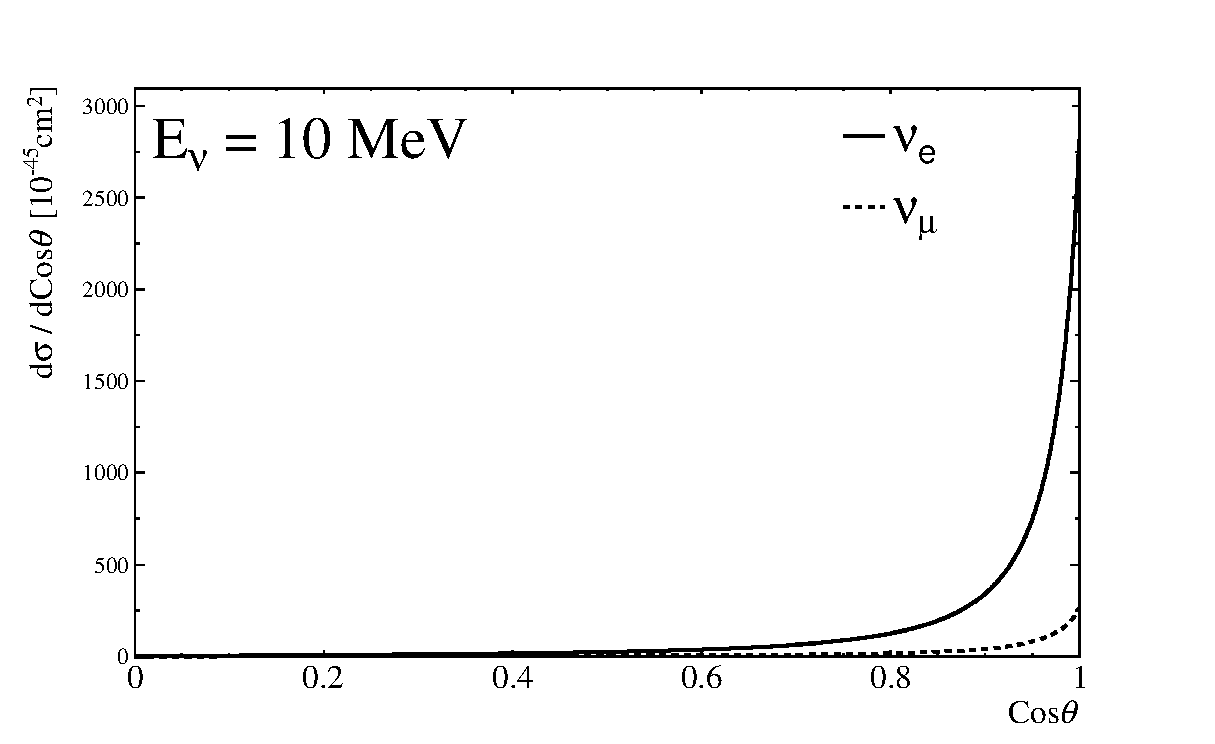
\includegraphics[width=\textwidth]{neutrino_xsec_energy}
\caption[ES Recoil Energy Cross-Section]{}
\label{}
\end{subfigure}
\hfill
\begin{subfigure}[b]{0.48\textwidth}
\centering
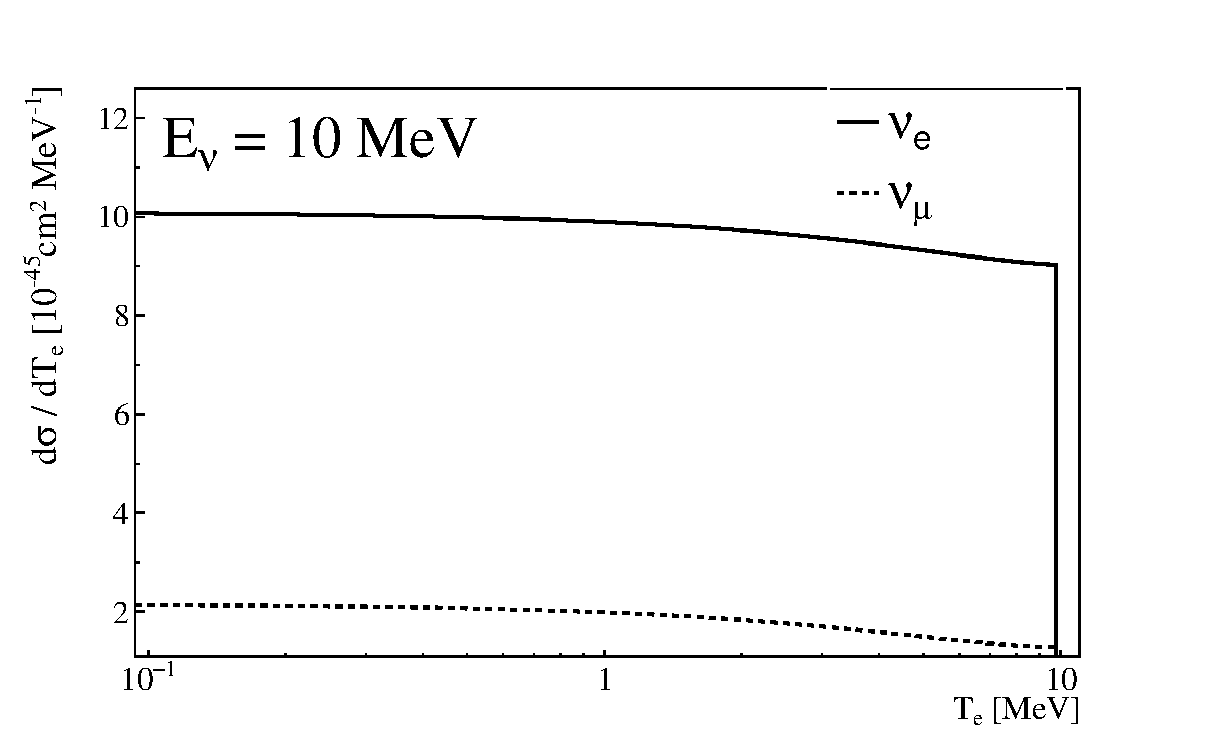
\includegraphics[width=\textwidth]{neutrino_xsec_angular}
\caption[ES Angular Cross-Section]{}
\label{}
\end{subfigure}
\caption[Neutrino-Electron ES Cross-Sections]{The electron recoil\,(a)
cross-section and electron angular\,(b) cross-section for neutrino-electron
elastic scattering with a 10\,MeV incoming neutrino energy.}
\label{fig:es_xsec}
\end{figure}


Figure~\ref{fig:es_xsec} shows the differential cross-sections for a 10\,MeV neutrino.
The fact that the scattering cross-section is peaked near $\cos\theta=1$
is very useufl for neutrino experiments; the observed electron direction
will almost always be nearly co-linear with the incoming neutrino direction.
Unforunately, since the cross-section is nearly flat in $T_{\mathrm{e}}$
the electron energy provides almost no information about the incoming neutrino
energy.
The kinematics and cross-section of the out-going neutrino is also
well predicted with respect to $\cos\theta$, however the out-going
neutrino is typically of little interest because it cannot be detected.

Experimentally neutrino elastic scattering has been studied in a number
of venues historically and recently~\cite{reines2, es_measurement, nutev}.
Famously the first experimental evidence for the $Z$ boson came from
the observations of neutrino elastic scattering at the
Gargamelle experiment~\cite{gargamelle}.
It's also been a useful detection method for water-cherenkov solar
neutrino experiments because the directionality of the interaction
allow events that originate from the Sun to be identified~\cite{sno_first,
kamiokande, superk_first_solar}.

\section{Neutrino Oscillations}
\label{sec:neut_osc}
Neutrino oscillation is a phenomena of massive neutrinos, and it's observation
is currently the only evidence that neutrinos do indeed have mass.
Neutrino oscillation results from the fact that neutrino flavors do not have
well defined masses, instead neutrino flavor states are a quantum superposition
of neutrino mass states.
And conversely, mass states can be described as a superposition of flavor states.
This can be stated more precisely as
\begin{equation}
    \ket{\nu_{i}} = U_{i\ell}\ket{\nu_\ell}
\end{equation}
Where $\ket{\nu_\ell}$ represents the neutrino flavor states, $\ket{\nu_i}$
represents the mass states, and $U_{i\ell}$ describes the mixing of these
states.
$U$ is known as the Pontecorvo-Maki-Nakagawa-Sakata (PMNS) matrix,
and it is exactly analogous to the Cabibbo-Kobayashi-Maskawa (CKM) matrix used
to describe quark mixing.
In the simplest case where the weak states and the mass states are the same
$U$ would just be the identity matrix.
Under the assumption that there are three flavor states and three mass states
$U_{i\ell}$ must be unitary so that the probability of observing
a neutrino in any state is never less than one.
It is known from observations of Z boson decay products that
there are only three ``active'' neutrino flavors~\cite{Zdecay}.
Where active means that the neutrino participates in
weak interactions.
It's possible there there is a neutrino that does not interact
weakly, this is referred to as a sterile neutrino and is the
subject of a number of experimental searches~\cite{prospect, lsnd, miniboone, jsns2}.
If there were a sterile neutrino state the $3\times3$ PMNS matrix would
no longer be unitary.

It is typical to characterize $U$ with three angles
($\theta_{12}$, $\theta_{13}$, $\theta_{23}$) and a CP violating
phase $\delta_{cp}$. Doing so allows for the general SU(3) mixing matrix to
be decomposed into two SO(2) matrices and one SU(2) matrix,
$$U_{12} =
\begin{bmatrix}
    \cos\theta_{12} & \sin\theta_{12} & 0  \\
    -\sin\theta_{12}& \cos\theta_{12} & 0  \\
    0 & 0 & 0  \\
\end{bmatrix},
$$
$$
U_{13} =
\begin{bmatrix}
    \cos\theta_{13} & 0 & \sin\theta_{13}e^{-i\delta_{cp}}\\
    0 & 0 & 0  \\
    -\sin\theta_{13} e^{-i\delta_{cp}} & 0 & \cos\theta_{13}  \\
\end{bmatrix},
$$
$$
U_{23} =
\begin{bmatrix}
    0 & 0 & 0  \\
    0 & \cos\theta_{23} & \sin\theta_{23} \\
    0 & -\sin\theta_{23} & \cos\theta_{23}   \\
\end{bmatrix}.
$$
The product of these matrices produces the full mixing matrix,
$U = U_{23}U_{13}U_{12}$.

The mixed nature of neutrino flavor and mass states gives rise to oscillations
in the flavor content of propagating neutrinos.
By definition the neutrino mass states are eigenstates of the vacuum Hamiltonian
\begin{equation}
    H\ket{\nu_{i}} = E_{i}\ket{\nu_{i}}\text{,}
\end{equation}
where the energy is given by the standard relativistic energy equation,
\begin{equation}
    E_{i} = \sqrt{{(p_{i}c)}^{2} + {(m_{i}c^{2})}^2}\text{.}
\end{equation}
It is typical to make the assumption that all neutrino mass states have the same
momentum, $p_{i} = p$.
The equal momentum assumption allows for a straightforward derivation of the
correct description of neutrino oscillations, but it is not well motivated.
A discussion of the equal momentum assumption and its validity
is available in Ref~\cite{neutrino_osc_subtleties}.

Applying Schrodinger's equation,
\begin{equation}
    i\frac{d}{dt}\ket{\nu_{i}(t)} = H\ket{\nu_{i}(t)} = E_{i}\ket{\nu_{i}(t)}\text{,}
\end{equation}
results in,
\begin{equation}
    \ket{\nu_{i}(t)} = e^{-iE_{i}t}\ket{\nu_{i}(t=0)}\text{.}
    \label{eqn:mass_state_tevol}
\end{equation}

This time evolution of mass eigenstates can be used to then describe the state
of a neutrino that is created in a electron flavor eigenstate.
\begin{equation}
\ket{\nu(t=0)} = \ket{\nu_{e}} = U_{1e}\ket{\nu_1} + U_{2e}\ket{\nu_{2}} + U_{3e}\ket{\nu_{3}}
    =\sum_{i=1}^{3}U_{ie}\ket{\nu_{i}}
\end{equation}

Each of the mass states' time evolution can be immediately written down from
Equation~\eqref{eqn:mass_state_tevol},
\begin{equation}
    \ket{\nu(t)} = \sum_{i=1}^{3} U_{ie}e^{-iE_{i}t}\ket{\nu_{i}}\text{.}
    \label{eqn:e_state}
\end{equation}

From Eqn.~\eqref{eqn:e_state} the quantity that's often of the most interest
is the survival probability, defined as
\begin{equation}
    P_{ee}(t) = \abs{\braket{\nu_{e}}{\nu(t)}}^{2}\text{.}
\end{equation}
$P_{ee}(t)$ can be understood as the probability that a neutrino, produced in
an electron flavor state, will be detected as an electron flavor state a time
$t$ later.
The survival probability for the state given in Eqn.~\eqref{eqn:e_state} is
\begin{equation}
    P_{ee}(t) = \sum_{i,j}\abs{U_{ei}}^2\abs{U_{ej}}^2e^{-i(E_{i} - E_{j})t}\text{.}
\end{equation}
It is useful to separate out the terms where $i=j$,
\begin{equation}
    P_{ee}(t) = \sum_{i}\abs{U_{ei}}^4 + \sum_{i,j\text{, }j \ne i}
    \abs{U_{ei}}^2\abs{U_{ej}}^2e^{-i(E_{i} - E_{j})t}\text{.}
\end{equation}
Here we can see there are terms that oscillate with time, and terms that do
not.

A few more simplifications are commonly done, using the equal momentum
assumption mentioned earlier and the fact the neutrino rest mass is
very small, the energy differences can be simplified,
\begin{equation}
    E_{i} - E_{j} = \sqrt{p^{2} + m_{i}^{2}} - \sqrt{p^{2} + m_{j}^{2}} \approx
    p^{2} - p^{2} + \frac{m_{i}^2}{2p} - \frac{m_{j}^2}{2p}\text{.}
\end{equation}
To good approximation $p=E$, so
\begin{equation}
    E_{i} - E_{j} = \frac{\Delta m^{2}_{ij}}{2E}\text{,}
\end{equation}
where the definition of the mass-squared splittings is used,
\begin{equation}
    \Delta m^{2}_{ij} = m^{2}_{i} - m^{2}_{j}\text{.}
\end{equation}

The final simplification is to assume that the neutrino is moving very close
to the speed of light, therefore any flavor oscillations over time will also
occur at a distance $L$ from the neutrino's creation.
All this gives
\begin{equation}
    \label{eqn:pee_adiabatic}
    P_{ee}(L,E) = \sum_{i}^{3}\abs{U_{ei}}^4 +
    \sum_{i,j\text{, }j \ne i}^{3}
    \abs{U_{ei}}^2\abs{U_{ej}}^2e^{-i\left(\frac{\Delta m^{2}_{ij}}{2E}L\right)}\text{.}
\end{equation}
For the mixing parameters given in~\cite{PDG2016} the average survival probability
for a electron neutrino is $P_{ee} = 55.8\%$.

With the exception of the CP violating phase $\delta_{cp}$, all mixing
parameters and mass-squared splitting have been measured experimentally~\cite{pdg_globalfit}.
None of the parameters are not predicted from the standard model, so are theoretically
unconstrained.
The measurements of the mass-squared splittings and
other parameters are discussed in Sec.~\ref{sec:experiments}.
The absolute mass of each neutrino state is not yet known.
There are upper limits placed on the sum of the neutrino masses from
observations of tritium decay~\cite{troitsk_mass}, and from cosmological
observations and modelling~\cite{cosmological_neutrino_mass}.

Also unknown is the ``hierarchy'' of the neutrino masses, i.e.\ which
mass states are heavier or lighter than the others.
Solar neutrino measurements have established that the $\nu_{2}$ state
is more massive than the $\nu_{1}$ state~\cite{sno_first, sno_combined}, but so far no experiment has been
able to resolve if $\nu_{3}$ is more or less massive than $\nu_{1}$ and $\nu_{2}$ states~\cite{vogel_hierarchy}.
The case where the $\nu_{1}$ state is the lightest is referred to as the
``normal hierarchy'' because then neutrino mass state have the same
ordering as the charged leptons;
the case where $\nu_{3}$ is the least massive neutrino is known as the
 ``inverted hierarchy'', because then the neutrino mass states are opposite
 that of the charged lepton states.
 Experimental measurements and cosmological consdierations currently prefer
 the normal hierarchy over the inverted hierarchy at approximately $2.4\sigma$ statistical
 significance~\cite{nu_fit}

This model of neutrino mixing assumes that neutrinos are Dirac, as opposed to
Majorana. In the case that the neutrino is a Majorana particle the PMNS matrix
gains two additional complex ``Majorana'' phases, similar to the CP violating
phase $\delta_{CP}$.
However, neutrino oscillation observables, such as the survival and transition
probability, are in general not effected by the Majorana phase~\cite{majorana_mixing}.
Therefore it is acceptable to ignore the presence of Majorana phases in typical 
neutrino mixing calculations.

\subsection{Matter Enhanced Oscillations}
When neutrino propagate through matter, as opposed to vacuum, its oscillation is altered.
The local density of other particles modifies the vacuum Hamiltonian,
adding a weak interaction potential.
The interaction comes primarily from a neutral current interaction of the form
shown in Fig.~\ref{fig:nuclear_nc}, and a flavor dependent charged current interaction shown in
Fig.~\ref{fig:nuclear_cc} and the  neutrino elastic scattering potential shown in
Fig.~\ref{fig:ES_CC} and Fig.~\ref{ES_NC}.
Nearly all normal matter contains a much higher density of electrons
than the other flavors of charged lepton, so the charged current reaction
elastic scatter modifies the electron neutrino potential and not the potential for the muon
or tau neutrino.
The result is that the electron density through which a neutrino propagates
can modify the effective mass-splitting and mixing angle for the electron
neutrino.
For a given neutrino energy $E_{\nu}$ there exists an electron density for which
the effective mixing angle is maximal, this is known as the resonant density~\cite{wolfenstein_osc, ms_oscillation}.
This resonance is important for solar neutrinos and will be discussed more in
the next section.

The adabiticity of neutrino oscillation refers if mass state composition
of a neutrino state changes or not, if it does change then the neutrinos
oscillation is non-adiabatic.
A specific example is if a neutrino state is a pure vacuum mass-1
state,
\begin{equation*}
    \ket{\Psi_{\nu}} = \ket{\nu_{1}}
\end{equation*}
suddenly enters a region of significant matter density where the mass states
are now $\ket{\nu_{k}^\prime}$.
The neutrino state does not have time to evolve at all so the state
does not change, but it is not longer a pure eigenstate of the mixing
Hamiltonian,
\begin{equation*}
    \ket{\Psi_{\nu}} = \ket{\nu_{1}} = \sum_{k=1}^{3} \braket{\nu_{k}^\prime}{\nu_{1}}\ket{\nu_{k}^\prime}\text{.}
\end{equation*}
Since the neutrino is no longer in a pure eigenstate the state will
now oscillate.

In contrast if the neutrino slowly enters the region of significant matter
density more slowly, then the neutrino state will smoothly evolve with the
eigenstate, $\ket{\nu_{1}} \rightarrow \ket{\nu_{1}^{\prime}}$.
And so the final state of the neutrino in the adiabatic case will be,
\begin{equation*}
    \ket{\Psi_{\nu}} = \ket{\nu_{1}^{\prime}}\text{.}
\end{equation*}

The adiabaticity of neutrino evolution will be discussed further in
Chapter~\ref{sec:chameleons}.

\section{Solar Neutrinos}
\begin{figure}[htbp]
\centering
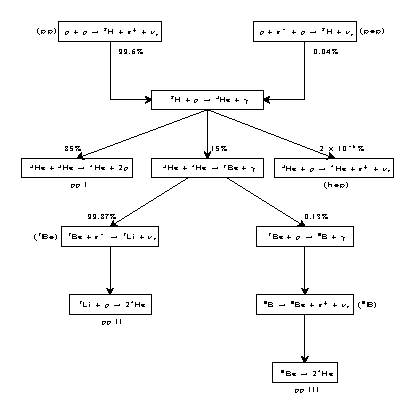
\includegraphics[width=0.8\textwidth]{pp_chain}
\caption[$pp$ Chain Solar Reactions]{The $pp$ chain reactions with
branching ratios for the Sun, values from~\cite{bahcall_book}.}
\label{fig:pp_chain}
\end{figure}
\begin{figure}[htbp]
\centering
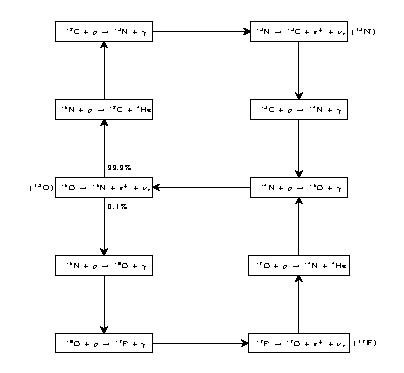
\includegraphics[width=0.8\textwidth]{cno_cycle}
\caption[CNO Cycle Solar Reactions]{The CNO cycle reactions with
branching ratios for the Sun, values from~\cite{bahcall_book}.}
\label{fig:cno_cycle}
\end{figure}
Nuclear reactions in the core of the Sun provides the main fuel for
stellar burning, and prevents the Sun from undergoing gravitational
collapse~\cite{XXX}. %XXXTODO find a  source like Bethe or something
There exists two separate chains of nuclear reactions that are present in typical
stellar conditions, the $pp$-chain and the CNO-cycle~\cite{bahcall_solar_neutrinos_theory}.
Figure~\ref{fig:pp_chain} and~\ref{fig:cno_cycle} shows these two reaction chains.
For the Sun the $pp$ chain
provides 99\% of the generated nuclear energy, and the CNO-cycle provides the remaining
1\%. For stars significantly more massive than the Sun, the CNO-cycle is the
main energy generating mechanism.

\begin{figure}[htbp]
\centering
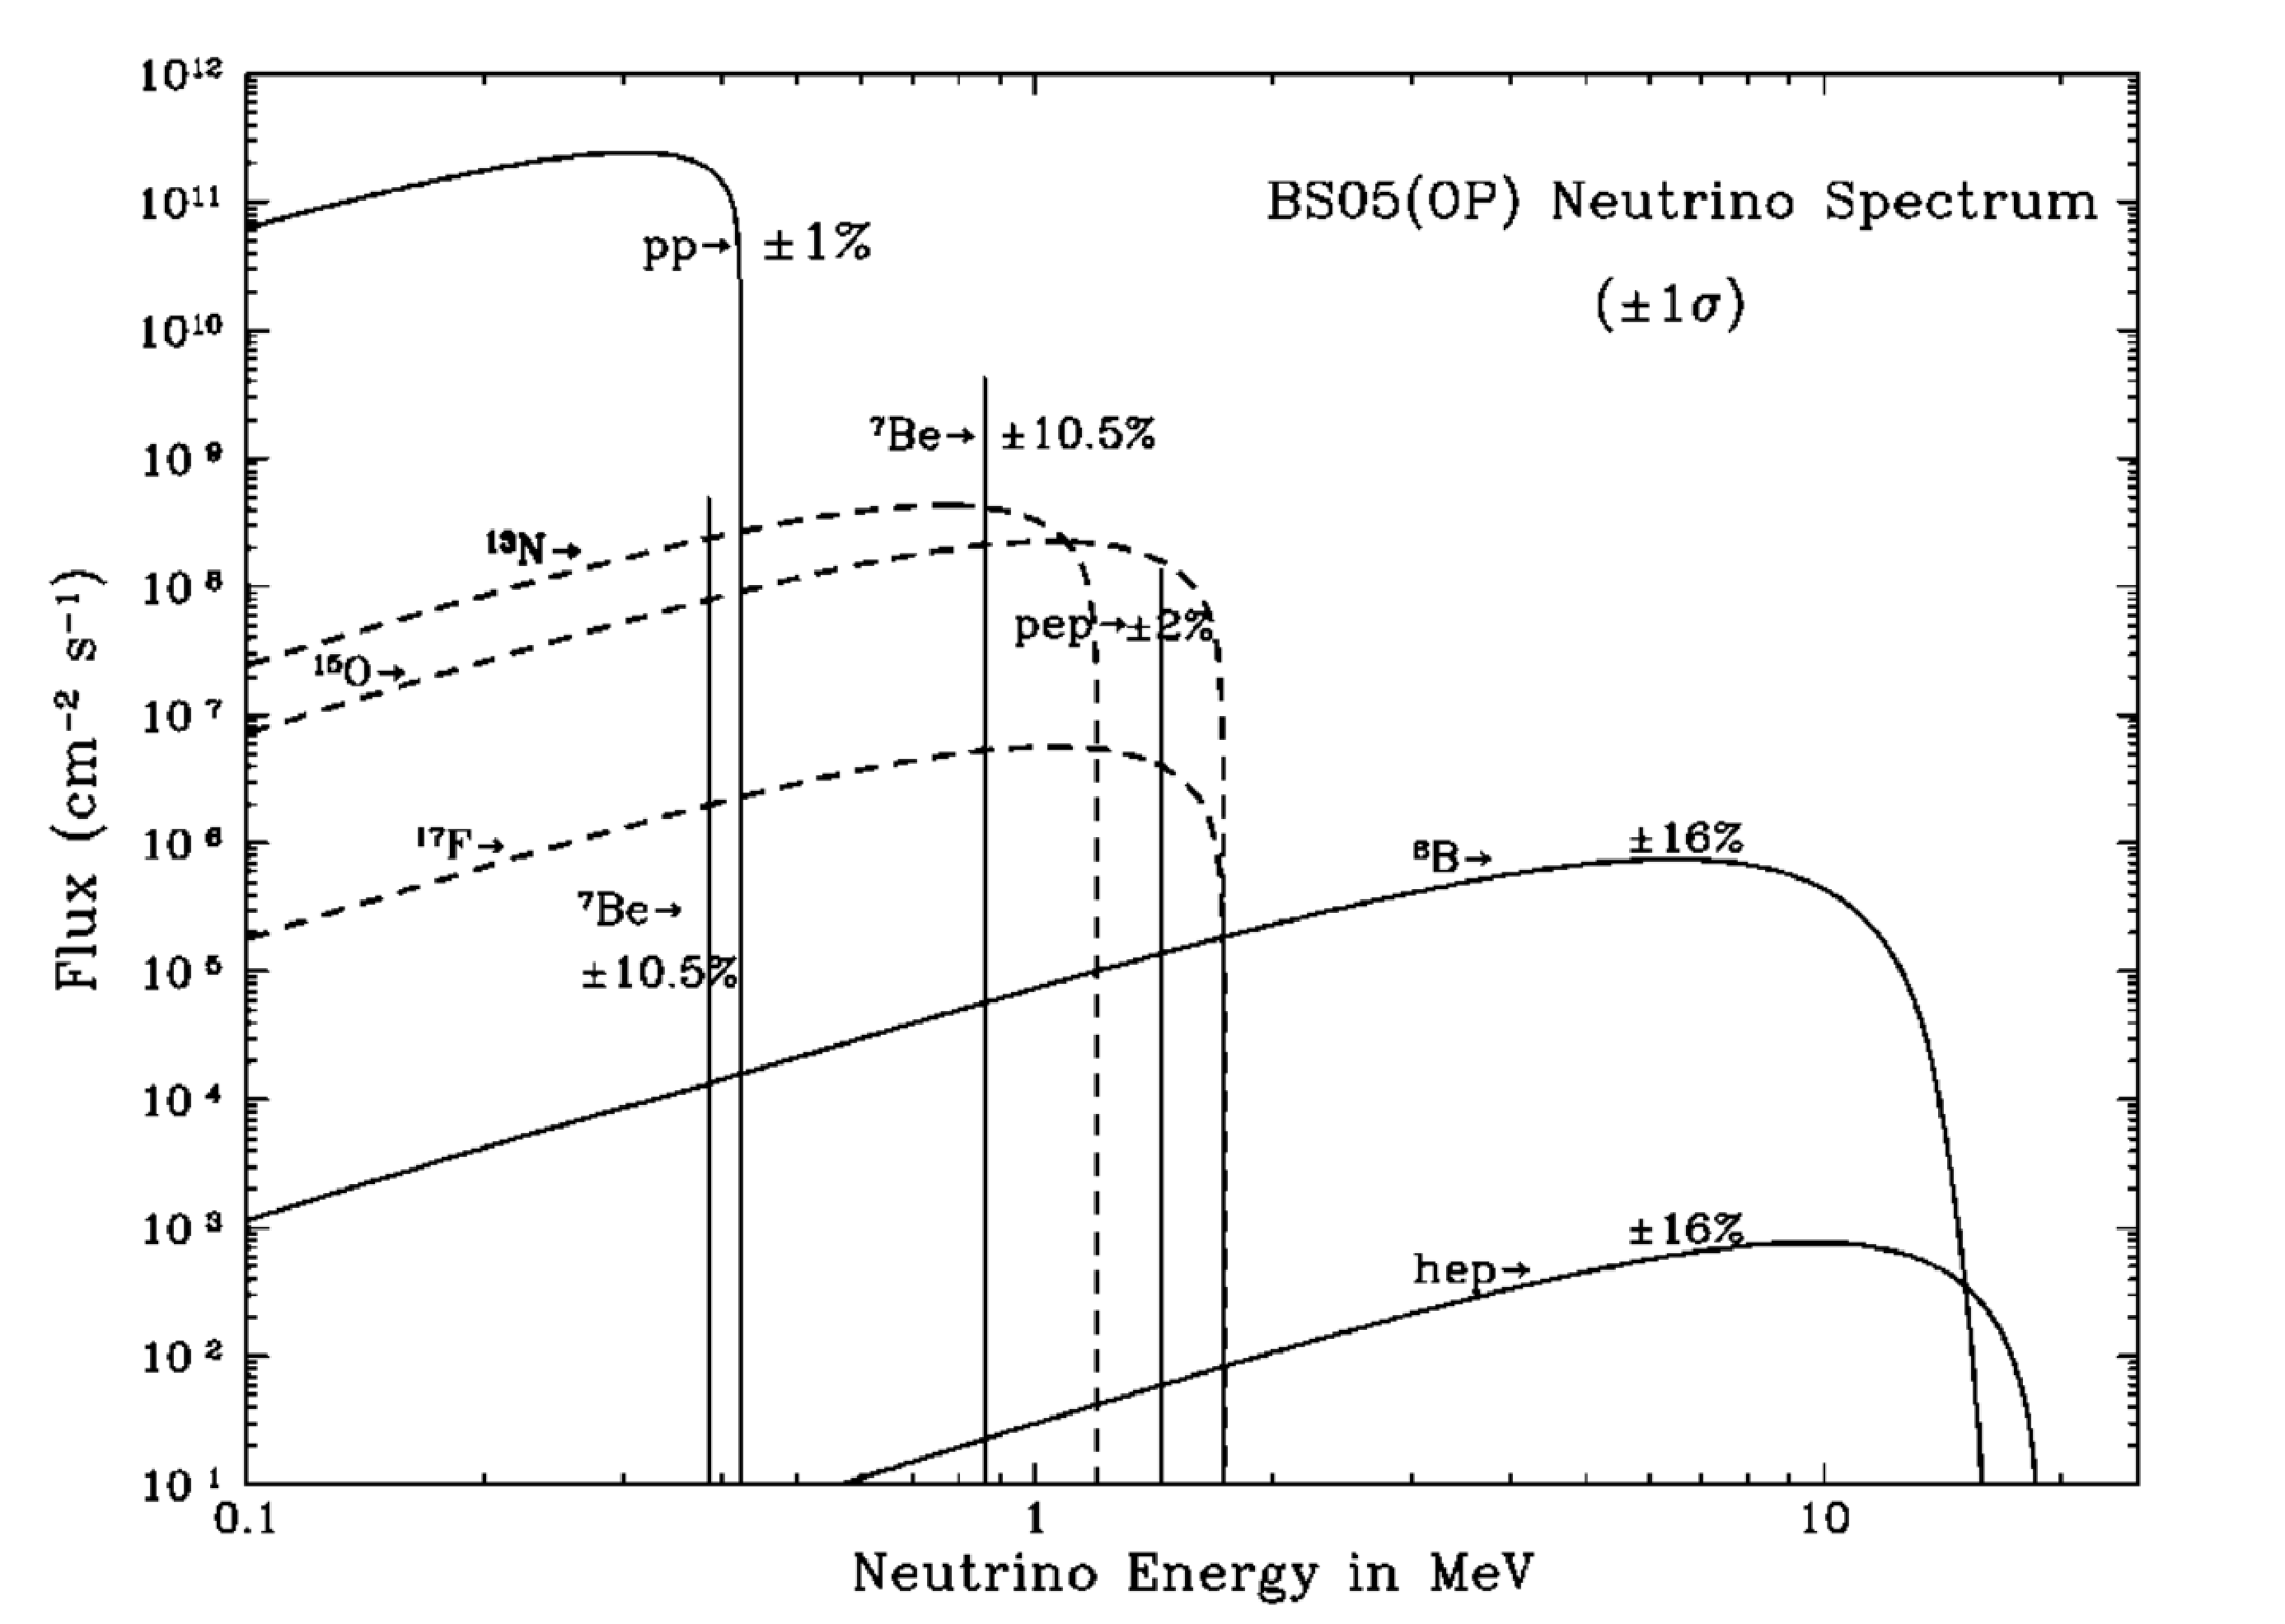
\includegraphics[width=0.6\textwidth]{bs05op_spectrum}
\caption[Solar Neutrino Spectrum]{Energy spectrum for neutrinos from
the Sun with normalization uncertainties. Figure from~\cite{bs_ssm}.}
\label{fig:bs05_spectrum}
\end{figure}

Within the $pp$-chain there are five processes that produce neutrinos.
Since the Q-value the processes in the $pp$ chain are all below the rest mass
of a muon or tau, the only charged lepton generated is electrons. And so from
lepton flavor conservation only electron flavor neutrinos are generated.
And because the neutrino producing processes are all fusion reactions or
$\beta^{+}$ decay, only neutrinos are produced and not any anti-neutrinos.
These neutrinos are produced with an energy spectrum shown in Fig.~\ref{bs05_spectrum}.

The $hep$ and $\ce{^{8}B}$ reactions produce neutrinos with the highest
energies. Since the $hep$ reaction branching ratio is so low the flux
of $hep$ neutrinos is also very low compared to that of $\ce{^{8}B}$ neutrinos;
the $hep$ flux is expected to be approximately $0.15\%$ of the $\ce{^{8}B}$ flux.
So for water-Cherenkov detectors that have a typical threshold of a few MeV, $\ce{^{8}B}$ neutrinos
are the primary source of detectable solar neutrinos.

The uncertainty on the predicted $\ce{^{8}B}$ flux is relatively large, this comes mostly
from the uncertainty on the cross-sections and how those cross-sections change with
temperature, and uncertainties on the temperature profile within the core of the sun.
And since the $\ce{^{8}B}$ reaction has five preceding reactions the uncertainty on
 those reactions are part of the uncertainty on the $\ce{^{8}B}$ flux.

The uncertainty on the $pp$ and $pep$ neutrinos is much lower for two reasons. First, because
they are at early stage of the reaction chain, so their reaction rate is not dependent on any
other preceding interaction. The $pp$ reaction is also the main energy generating mechanism
for the Sun, so measurements of the total solar luminosity provide strict constraints on the
$pp$ flux as well.

Predictions for solar neutrinos rely heavily on solar modelling, which in turn
is constrained by observations of the Sun.
Detailed solar models will simulate the evolution of the Sun from a proto-star
with a given mixture of chemical abundances and produce predictions for
what we would expect to observe today.
Following this procedure a temperature and density profile for the Sun is determined
which in turn leads to predictions for solar neutrino production.
For this work the BS05OP~\cite{bs_ssm} predictions are typically used.
Figure{XXX} shows the solar neutrino production distribution within the Sun.

Photospheric and helioseismological measurements of chemical abundances provide
input for solar models.
%and helioseismological measurements of the speed of sound in or across the Sun.  The speed of sound measurements can be used to estimate the require chemical composition.
%From this procedure the standard chemical abundances were determined~\cite{gs98}.
There are two standard estimates for the solar chemical abundances,
GS98~\cite{gs98} and AGS~\cite{ags}.
The most significant discrepancy between the two models is in the value
for the solar metallicity, the AGS prediction for the metallicity is
lower by roughly a factor of two.
The AGS estimates make use of a 3-dimensional model of the solar photosphere,
as opposed to the GS98 estimates which use a 1-dimensional model, however
the AGS model also produces discrepancies between photospheric measurements
and helioseismological measurements of the Sun~\cite{ags, bahcall01}.
The disagreements between the two models has become known as the
``Solar Metallicity Problem''.
For this work the GS98 values for chemical abundances is generally used if
both are not considered.

\subsection{Solar Neutrino Mixing}
Mixing for solar neutrinos is historically very important as it was
the measurements of solar neutrinos that provided the first evidence that
neutrinos mix at all~\cite{homestake,solar_nu_problem}.
Those measurements began the Solar Neutrino Problem, which wasn't solved
for nearly three decades and its eventual resolution by SNO and Super Kamiokande
led to the initial measurements of the neutrino mixing parameters~\cite{superk_atmospherics,
sno_second}.
Still today the Sun provides an unique source of neutrinos that travel through
densities and distances that cannot be produced by any other source, thus making
them a valuable object for study.

Neutrinos created in the solar core can experience significant mixing effects from local
electron density.
One of the most interesting aspects to neutrino mixing within the Sun is the MSW-effect,
at a specific electron density a resonance occurs and neutrinos are maximally mixed.
The condition for an MSW-resonance between any two matter states is given by
\begin{equation}
    N_{e} = \frac{\Delta m^{2} \cos2\theta}{2\sqrt{2}EG_{F}}\text{.}
\end{equation}
This condition is met for a 10\,MeV at a solar radius of XXX, for the mixing parameters
given in XXX %cite pdg probably.
For neutrinos below XXX\,MeV this condition is not met at any point within the sun,
and so those neutrinos do not experience the MSW resonance.
Once a neutrino created in the core of the sun has travelled past a solar radius of $\approx$XXX
the solar electron density has dropped far enough that matter effects are no longer significant
and neutrinos are effectively travelling through vacuum. Once in the vacuum mixing dominated region

The effect neutrino mixing has on the neutrino flux is typically summarized by the
$\ce{^{8}B}$ survival probability, $P_{ee}(E_{\nu})$ over the energy range $0-15\,MeV$,
shown in Fig~\ref{XXX}.

For solar neutrinos it's generally assumed that the neutrino states
will evolve adiabatically.
However, when the neutrino transitions through the MSW-resonance
the flavor composition of the mass states changes very rapidly,
so it's thought that this could lead to a non-adiabatic transition
between the mass-1 and mass-2 state.
For solar neutrinos the effect this transition would have on the
neutrino survival probability is characterized with $P_{jump}$,
\begin{equation}
    P_{jump} = \mathrm{exp}\left[-\dfrac{\pi}{2} \dfrac{\sin^{2}2\theta_{12}}{\cos2\theta_{12}}
               \dfrac{\frac{\Delta m^{2}_{21}}{2E}}{\frac{1}{N} \frac{dN}{dx}|_{x_{R}}}   \right]\cite{parke}\text{.}
\end{equation}
Where $x_{R}$ indicates the position at which the resonant density is crossed
and $N$ is electron density as a function of position.
For values of $\theta_{12}$ and $\Delta m^{2}_{21}$ near those determined by experimental
observation $P_{jump}$ is negligible.


\section{Neutrino Experiments}
\label{sec:experiments}
There's a long a diverse list of neutrino experiments that have contriubted to
our current understanding of neutrinos and neutrino oscillations.
I won't attempt to list them all here, but rather highlight the most immediatly
relevant to this work. A more compresive review can be found in \citep{FINDAREVIEW}.

\subsection{Homestake}
The first experiment to succesfully detect solar neutrinos was the Homestake
experiment.
The detector was composed of approximately 100000 gallons of dry cleaning fluid.
The choice of target was motivated by the high chlorine content in the cleaning
fluid. Neutrinos above an energy of XXX would interact with the chlorine via
beta decay, creating XXX. XXX would then decay to XXX with a half life of XXX.
Periodically $\ce{^{3}He}$ was bubbled through the
target liquid to extract the atoms of XXX that had been created. Once
extracted those atoms were observed with proportional counters to count the
number of XXX to XXX decays. The number of observed counts was proportional
to the solar neutrino interaction rate, and therefore the solar neutrino flux.

The homestake experiment ran from 1970 - 1990. %(XXX? is that right??)
The experiment was able to provide the first measurement of the solar neutrino
flux above XXX MeV. In 19XX they first reported a measure flux of
XXX, nearly a third of the expted rate which was XXX.
This deficiency became known as the solar neutrino problem, and it
was the first evidence for neutrino oscillation.
The deficiency was present across the entire lifetime of the Homestake experiment,
their final report flux was XXX.

\subsection{SNO}
\label{sec:sno}
The Sudbury Neutrino Observatory (SNO) is a water-Cherenkov detector located
roughly $2$\,km underground near Sudbury Ontario in Canada, it ran from
$1999$ to $2006$.
SNO was primarily a solar neutrino detector, it had the unique benefit of
being able to detect neutrinos through three different interaction channels,
each channel had it's own sensitivity to different flavor neutrinos.
This allowed for a measurment of the $^8B$ solar neutrino flux that was not
dependent on the flavor composition of the incoming neutrinos.
This was accoplished by using a heavy-water ($\ce{^{2}H_{2}O}$) target.
Heavy-water's primary neutrino interactions are the
electron scattering interaction (ES), a charged current nuclear reaction (CC),
and a neutral current nuclear reaction (NC).
%TODO add feynman diagrams for those reactions.
There exists both charged current and a neutral current versions of the
ES interaction; since electron neutrinos can interact through either
of the two where as muon or tau neutrinos can only elastic scatter throug the
neutral current version, the ES cross-section for electron neutrinos is larger
than the cross-section for muon and tau neutrinos.
The difference in cross-section is energy dependent, but it's roughly a factor
of 6 for solar neutrino energies. The neutral current and charged current ES reactions
are not treated seperately because there is no detectable signature that
would allow you to discrimate between the two.

The NC interaction on a deuteron can break apart the neutron and proton
that comprises the nucleus. $\nu_{e} + D -> p + n + \nu_{e}$.
The free-neutron can then capture on the deuterium forming tritium ($\ce{^{3}H}$)
and emitting an $XXX$\,MeV gamma. %TODO how often does it capture on oxygen?????
The NC reaction has no neutrino flavor preference, so a measure of the rate
of NC rate along with the process' cross-section provides a flavor independent
measurement of the solar neutrino flux.

The charged current interaction on a deuteron converts a neutron to a
proton and produces an electron.$\nu_{e} + D -> H + H + e^{-}$.
This reaction can only occur when the charged lepton and the neutrino are the same
flavor. So for typical matter this reaction only occurs for the electron flavor
neutrinos, and so it provides a measurement of the electron flavor content
of the solar neutrino flux.

SNO was able to seperate and count the events of each type of interaction,
providing them three independent measurements of solar neutrinos. And
the rates of each measurement had a different dependence on the flavor content
of solar neutrinos.


\subsection{Super Kamiokande}
Super Kamiokande (SuperK) is a 50\,kton cylindrical water cherekov detector.
It started running in $1996$ and has since made the most precise measurements of
atmospheric neutrinos and solar neutrinos so far.
It's the successor to the previous Kamiokande experiment, which was a significantly
smaller and had a higher energy threshold for detection.
SuperK can detect $\ce{^{8}B}$ solar neutrinos through only neutrino-electron elastic scattering,
they do not use a $\ce{D_{2}O}$ target and so are not sensitive to the
nuclear interactions that SNO used.
Their extremely large detector volume though provides them with far more exposure
than SNO could attain though. This results in a very precise measurement of the
elastic scattering rate.

The SuperK experiment seperates their dataset into 4 subsets, called
SuperK-I, SuperK-II, \textit{etc}. %TODO Roman numerals.
Each dataset covers several years of data taking.

\subsection{Borexino}
Borexino is 300\,ton spherical liquid scintillator detector~\cite{borexino_tdr}. Their detector
apparatus is similar to that of a water-Cherenkov detector, the significant difference
is that the water is replaced with pseudo-cumine, a liquid scintillator.
A charged particle moving through scintillator generates roughly 50-100 times
more light than a similar particle moving through just water.
Water-Cherenkov detector are typically limited in energy threshold
and energy resolution by the number of photons produced and detected, a liquid scintillator
detector solves this problem.  Scintillation light, unlike Cherenkov light,
is isotropic and provides no information about the direction the particle
was moving in.
\begin{figure}[htbp]
    \centering
    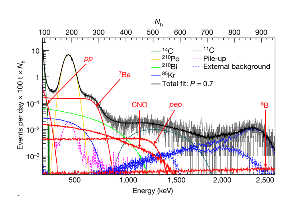
\includegraphics[width=0.75\textwidth]{borexino_spectrum}
    \caption[Borexino Spectrum] {Borexino's observed distribution of event energies with best fit
    signal and background model.
    $N_{h}$ is the number of prompt PMT hits.  Figure from~\cite{borexino_nature}.} %XXX Look up N_h to be sure
\label{fig:borexino_spectrum}
\end{figure}

Water-Cherenkov detector are able to measure solar neutrinos by correlating the
direction of detected events with the position of the sun. Since Borexino is not
able to determine the direction of events within their detector, they instead
perform a spectroscopic measurement. The measurement requires
all sources of backgrounds to be accounted for and constrained from \textit{ex-situ}
measurements. Figure \ref{fig:borexino_spectrum} shows the observed spectrum by Borexino and the
spectrums of the constituent solar fluxes and backgrounds.

Borexino took data from 2007 to 2016, with a pause in 2010 to remove source
of radioactive backgrounds and improve the radio-purity of their detector.
With that data they've produced measurements of neutrino fluxes from the $\ce{^{7}Be}$,
$\ce{pep}$, $\ce{pp}$, and $\ce{^{8}B}$; they've also placed upper limits on the flux
of neutrinos from the CNO cycle and from the $hep$ solar reaction.
They're currently the only experiment to have measured the $\ce{pp}$ and $\ce{pep}$ neutrino
fluxes.

$XXX$ FIND TABLE\\
show spectrum and table of results

\subsection{KamLAND}
The Kamioka Liquid Scintillator Antineutrino Detector (KamLAND) is a liquid-scintillator detector.
Its primary physics goals were the detection of reactor anti-neutrinos via
inverse beta-decay (IBD),
but the experiment is also sensitive to solar neutrinos.
Performing a fit to the observed energy spectrum they were able to measure
the flux of $\ce{^{7}Be}$ and $\ce{^{8}B}$ solar neutrinos.
The $\ce{^{8}B}$ flux is reported as the ``elastic-scattering'' flux $\Phi_{ES}$, the flux of
pure electron flavor neutrinos that would produce the observed event rate.
They measure $\Phi_{ES\mathrm{,}\ce{^{8}B}} = 2.77 \pm 0.26(\mathrm{stat.}) \pm 0.32(\mathrm{syst.}) \times 10^6 \mathrm{cm}^{-2}\mathrm{s}^{-1}$~\cite{kamland_b8}.
KamLAND's reported $\ce{^{7}Be}$ flux, accounting for oscillation effects,  is
 $\Phi_{\ce{^{7}Be}} = (5.82\pm 1.02)\times10^{9} \mathrm{cm}^{-2}\mathrm{s}^{-1}$~\cite{kamland_be7}.


\begin{figure}[htbp]
\centering
\begin{subfigure}[b]{0.48\textwidth}
\centering
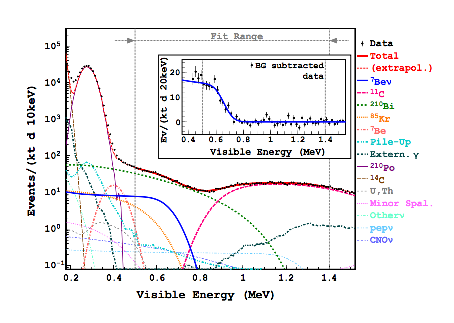
\includegraphics[width=\textwidth]{kamland_be7_spectrum}
\caption{}
\label{fig:kamland_be7}
\end{subfigure}
%\hfill
\begin{subfigure}[b]{0.48\textwidth}
\centering
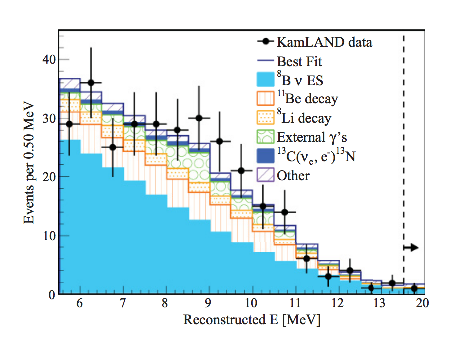
\includegraphics[width=\textwidth]{kamland_b8_spectrum}
\caption{}
\label{fig:kamland_b8}
\end{subfigure}
\caption{The observed reconstructed event energy spectrum for the Kamland Be7 flux measurement (a)
  and the 8B flux measurement (b). Figures from~\cite{kamland_be7} and~\cite{kamland_b8}.}
\label{fig:kamland_spectrum}
\end{figure}

Interestingly, KamLAND's reactor neutrino measurements~\cite{kamland_reactor} are
more relevant to the study of solar neutrinos than their solar neutrino measurements.
The long baseline (\urltilde180\,km) and low energy (\urltilde3\,MeV) of reactor neutrinos provides
unique sensitivity to $\Delta m^{2}_{21}$.
Other reactor neutrino experiments, such as Daya Bay, RENO, \& Double Chooz,
are primarily sensitive to neutrinos with too short a baseline to be strongly
affected by $\Delta m^{2}_{21}$.

\begin{figure}[htbp]
  \centering
  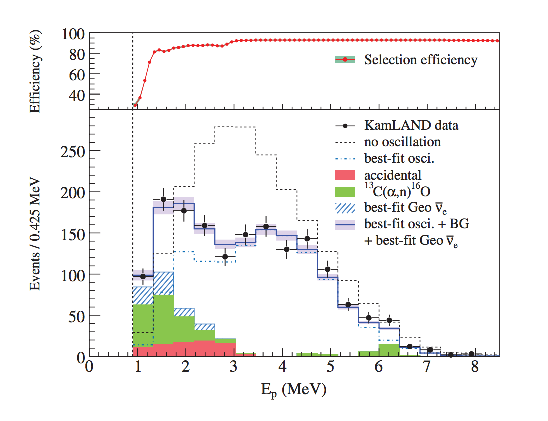
\includegraphics[width=0.75\textwidth]{kamland_reactor_spectrum}
  \caption[Kamland Reactor Spectrum]{Reactor anti-neutrino energy spectrum observed by KamLAND.
                                    Figure from~\cite{kamland_reactor}.}
  \label{fig:kamland_reactor}
\end{figure}

Figure~\ref{fig:kamland_reactor} shows reactor anti-neutrino energy spectrum measured
by the KamLAND experiment, with the best fit mixing parameters compared to the
expected spectrum with no oscillations.
From this measurement a best fit value of $\Delta m^{2}_{21} = 7.58^{+0.14}_{-0.13}(\mathrm{stat.})^{+0.15}_{-0.15}(\mathrm{syst.}) \times 10^{-5}$\,eV
and $\tan^{2} \theta_{12} = 0.56^{+0.10}_{-0.07}(\mathrm{stat.})^{+0.10}_{-0.06}(\mathrm{syst.})$ was determined.

The value for $\Delta m^{2}_{21}$ measured by KamLAND is in disagreement with the value extracted
by solar experiments, although it cannot be ruled out that the disagreement
is a result of a statistical fluctuation. This discrepancy will be discussed further
in section~\ref{sec:chameleons}.
